% PX4 SITL validation (included by report.tex)
\section{PX4 SITL validation and sim-to-sim analysis}\label{sec:sitl}
The exported policies were flown as PX4 offboard controllers against PX4~v1.16.2 software-in-the-loop (SITL) with the
Gazebo Harmonic \texttt{x500} model, whose rotor, motor and inertia parameters equal the quadsim X500 preset. SITL
replaces quadsim's rigid-body engine (PhysX $\to$ gz-physics), its onboard controllers (simulated rate PID and velocity
cascade $\to$ PX4 \texttt{mc\_rate\_control}, \texttt{mc\_pos\_control} and the control allocator) and its estimator model
(noise model $\to$ EKF2 fusing simulated IMU, GNSS, barometer and magnetometer), and adds the real deployment software
path (ROS~2 node, uXRCE-DDS, PX4 time synchronization). Differences between the two simulators therefore expose the
assumptions of the training environment that a real flight would also violate. Every experiment is scripted and
re-runnable (\texttt{ros2/px4\_sitl/setup\_px4\_sitl.sh}, \texttt{scripts/sitl/}); all reported numbers are computed by
the same unit-tested functions (\texttt{quadsim.deploy.closed\_loop\_metrics}) for quadsim and SITL.

\subsection{Setup and deployment pipeline}
\begin{figure}[h]\centering
\begin{tikzpicture}[node distance=4mm and 7mm, every node/.style={font=\footnotesize},
  box/.style={draw, rounded corners=2pt, align=center, minimum height=9mm, inner sep=3pt},
  arr/.style={-{Stealth[length=2mm]}, semithick}]
\node[box, fill=blue!6] (gz) {Gazebo Harmonic\\x500 (lockstep)};
\node[box, fill=blue!6, right=of gz] (px4) {PX4 v1.16.2\\EKF2, rate / velocity\\control, allocator};
\node[box, fill=orange!8, right=of px4] (dds) {uXRCE-DDS\\agent};
\node[box, fill=green!8, right=of dds] (bridge) {\texttt{quadsim\_px4\_bridge}\\\texttt{OffboardPolicy} + ONNX\\50\,Hz};
\node[box, fill=gray!8, below=of bridge] (scan) {virtual 2-D LiDAR\\(navigation)};
\node[box, fill=gray!8, below=of dds] (harness) {scenario harness\\(arm, hand-over,\\recording)};
\draw[arr] (gz) -- (px4); \draw[arr] (px4) -- node[above]{odometry} (dds); \draw[arr] (dds) -- (bridge);
\draw[arr] (bridge.south west) ++(0,0.1) -- ++(-0.3,-0.1) |- node[pos=0.25,left]{} (dds.south east);
\draw[arr] (scan) -- node[right]{\texttt{LaserScan}} (bridge);
\draw[arr] (harness) -- (dds);
\end{tikzpicture}
\caption{SITL loop. The bridge receives \texttt{VehicleOdometry} (EKF2, NED/FRD) and publishes
\texttt{OffboardControlMode} plus \texttt{VehicleRatesSetpoint} (CTBR policies) or \texttt{TrajectorySetpoint}
(velocity policies). The harness takes off with PX4, calibrates the thrust map, hands over to the policy, applies the task
and records odometry, simulator ground truth and commands in one time base.}
\label{fig:sitl}
\end{figure}
PX4 runs its EKF2 and controllers unmodified with airframe defaults, except \texttt{NAV\_DLL\_ACT}=0 (no ground
station) and \texttt{EKF2\_GPS\_DELAY}=0 (\cref{sec:sitl-est}). The only change to PX4 is SITL instrumentation that
exports the gz ground truth over DDS for evaluation. The bridge's per-step logic is the ROS-free class
\texttt{quadsim.deploy.offboard.OffboardPolicy}: it rebuilds the training observation of each task (hover goal; tracking
reference $t+\{0,\dots,1\}$\,s generated onboard; waypoint sequence with the training switching rule; navigation goal plus
the 32-ray range ring resampled from any \texttt{LaserScan}) and is checked against the simulator in closed loop
(observation error $\le7.5\times10^{-6}$ for all four tasks, ONNX vs PyTorch success within 3 points; generalized M6
test). A scenario starts with a PX4 take-off and Hold; the goal / reference / course is defined from the current pose and
the policy takes over in OFFBOARD; after the task PX4 takes back control and lands.

\textbf{Thrust map.} PX4 expects a normalized thrust $u\in[0,1]$. For gz \texttt{x500} the ESC maps $u$ to
$\omega=\omega_{\min}+(\omega_{\max}-\omega_{\min})u$ and the thrust is $T=4k_f\omega^2$, i.e.\ $T/T_{\max}=c(u)=(0.15+0.85u)^2$.
The documented calibration (linear map $u=s\,C/T_{\max}$ with $s=u_h/(mg/T_{\max})$ from PX4's hover-thrust estimate $u_h$)
is exact only at hover; there the true local gain exceeds the linear map's by
$\frac{c'(u_h)}{c(u_h)/u_h}=\frac{2\cdot0.85\,u_h}{0.15+0.85u_h}=1.61$ ($u_h=0.7295$). The bridge therefore also supports an
exact curve map $u=c^{-1}(s\,C/T_{\max})$ with $s=c(u_h)/(mg/T_{\max})$ (\texttt{ThrustCurve}); the calibrated
$s=1.0016$ shows that the gz model and the quadsim preset agree on hover thrust within \SI{0.2}{\percent}.

\textbf{Identification tools.} Command$\to$response dynamics are identified from closed-loop flight data by an output-error
fit of a first-order-plus-dead-time model $Y(s)/U(s)=Ke^{-Ls}/(\tau s+1)$ (grid over $L$ and $\tau$, least squares for $K$,
zero-order-held commands); estimator lag by the shift minimizing $\mathrm{E}\|\hat x(t)-x(t-L)\|^2$; limit cycles by the
RMS and Welch-spectrum peak of body rate, collective command and vertical velocity. All are unit-tested on synthetic
signals with known parameters.

\subsection{Defects found by SITL}
\begin{itemize}
\item \textbf{Bridge never commanded.} PX4~1.16 versions some DDS topics (\texttt{VehicleStatus}$\to$
\texttt{/fmu/out/vehicle\_status\_v1}); the original node subscribed to the unversioned name, never saw OFFBOARD and
sent no set-point. Reproduced: PX4 accepted OFFBOARD for \SI{8}{s} without receiving a single set-point and the vehicle
drifted \SI{3.5}{m} on the last attitude-controller command. Topic names are now derived from the message versions.
\item \textbf{Failsafe could never trigger.} PX4 detects offboard loss only from the \texttt{OffboardControlMode}
heartbeat (\texttt{COM\_OF\_LOSS\_T}); the node published it before its stale-odometry and geofence checks. The heartbeat
is now sent only while the node can command; verified: after a geofence violation PX4 left OFFBOARD after
\SI{1.03}{s} and, without RC, landed.
\item Packaging (\texttt{setup.cfg}), a \emph{last-action} input containing never-applied commands before the hand-over,
NaN/frame checks of the odometry.
\item \textbf{Measurement artefacts.} PX4's gz ground-truth velocity and ``angular velocity'' are backward differences
(the latter of Euler angles); truth rates are recomputed by central differences of the ground-truth quaternions. rclpy's
multi-threaded executor dropped $\approx$35\,\% of the messages in the recorder (PX4 itself received every set-point).
\end{itemize}

\subsection{Estimator}\label{sec:sitl-est}
\Cref{tab:sitl-est} summarizes EKF2's error against the gz ground truth. In hover it is dominated by a per-flight bias
(2--4\,cm) and a slow, correlated component (std \SI{1.4}{cm}, correlation time 2--3\,s); the white part is
$\approx$\SI{1}{mm} and the attitude error $\approx$\SI{0.2}{mrad}. quadsim's v0 odometry model is the opposite: mostly
white (\SI{1}{cm} position, \SI{3}{cm/s} velocity, \SI{10}{mrad} attitude). In motion, EKF2 led the truth by
\SI{0.11}{s}: its default GNSS delay compensation (\texttt{EKF2\_GPS\_DELAY}=\SI{110}{ms}, correct for real receivers)
assumes a latency the gz GNSS does not have. Matching it (0\,ms) removed the lead and halved the truth-referenced
tracking error (14$\to$\SI{7}{cm}). These statistics define the EKF-like model of the v1 training distribution.
\begin{table}[h]\centering\small
\begin{tabular}{lc}\toprule
Quantity & PX4 EKF2 in SITL\\\midrule
Per-flight position bias $|\bar e_p|$ (x / y / z) [cm] & 1.8 / 1.8 / 3.9\\
Slow position error ($<$0.5\,Hz) std [cm] & 1.4 / 1.4 / 1.5\\
Slow position error correlation time [s] & 1.7 / 1.9 / 3.2\\
Fast position error std [mm] & 1.3 / 1.5 / 1.1\\
Velocity error std [cm/s] & 0.94 / 1.05 / 0.41\\
Velocity error correlation time [s] & 0.81 / 0.35 / 2.14\\
Roll / pitch error std [mrad] & 0.19 / 0.20\\
Circle flight, \texttt{EKF2\_GPS\_DELAY}=110\,ms: lag x / y [ms], RMS error [cm] & -110 / -99, 12.0\\
Circle flight, \texttt{EKF2\_GPS\_DELAY}=0\,ms: lag x / y [ms], RMS error [cm] & -3 / -1, 6.3\\
\bottomrule\end{tabular}
% 6 hover runs

\caption{PX4 EKF2 error vs gz ground truth (\texttt{scripts/sitl/estimator\_stats.py}, \texttt{docs/results/sitl\_estimator.json}).}
\label{tab:sitl-est}
\end{table}

\subsection{Hover and set-point steps}
The scenario of \cref{tab:sitl-hover} holds the hand-over pose for \SI{30}{s} (RMS over 10--30\,s), then steps the goal by
\SI{1}{m} in $x$ and in $z$; quadsim flies the same schedule with 64 environments starting at the goal.
\begin{table}[h]\centering\small
\resizebox{\linewidth}{!}{\begin{tabular}{lcccc}\toprule
Metric & quadsim nominal & SITL linear map (3) & SITL curve map (4) & SITL linear + geometry fix (2)\\\midrule
Hover RMS error, truth [cm] & 1.59 $\pm$ 0.46 & 4.12 $\pm$ 1.94 & 6.00 $\pm$ 1.11 & 4.71 $\pm$ 1.06\\
Hover RMS error w.r.t. estimate [cm] & 1.88 $\pm$ 0.02 & 1.02 $\pm$ 0.13 & 0.83 $\pm$ 0.04 & 1.01 $\pm$ 0.22\\
Estimate vs truth, hover RMS [cm] & 2.28 $\pm$ 0.31 & 3.84 $\pm$ 2.08 & 5.81 $\pm$ 1.19 & 4.51 $\pm$ 1.08\\
$x$ step w.r.t. estimate: rise 10--90\,\% [s] & 0.65 $\pm$ 0.01 & 0.54 $\pm$ 0.01 & 0.55 $\pm$ 0.01 & 0.54 $\pm$ 0.00\\
$x$ step w.r.t. estimate: settling (5\,cm) [s] & 1.07 $\pm$ 0.02 & 1.84 $\pm$ 0.02 & 1.86 $\pm$ 0.02 & 1.86 $\pm$ 0.02\\
$z$ step w.r.t. estimate: rise 10--90\,\% [s] & 0.63 $\pm$ 0.01 & 0.64 $\pm$ 0.01 & 0.64 $\pm$ 0.01 & 0.62 $\pm$ 0.02\\
$z$ step w.r.t. estimate: settling (5\,cm) [s] & 1.00 $\pm$ 0.03 & 1.07 $\pm$ 0.05 & 1.02 $\pm$ 0.02 & 1.07 $\pm$ 0.03\\
Rate cmd$\to$rate: delay roll [ms] & 13 $\pm$ 4 & 23 $\pm$ 1 & 31 $\pm$ 1 & 15 $\pm$ 5\\
Rate cmd$\to$rate: delay pitch [ms] & 13 $\pm$ 4 & 13 $\pm$ 2 & 10 $\pm$ 1 & 10 $\pm$ 2\\
Rate cmd$\to$rate: $\tau$ roll [ms] & 53 $\pm$ 2 & 47 $\pm$ 2 & 38 & 38 $\pm$ 3\\
Rate cmd$\to$rate: $\tau$ pitch [ms] & 52 $\pm$ 0 & 39 $\pm$ 1 & 42 $\pm$ 1 & 41 $\pm$ 3\\
Hover collective $a_0$ std & 0.174 $\pm$ 0.018 & 0.218 $\pm$ 0.139 & 0.005 $\pm$ 0.000 & 0.178 $\pm$ 0.174\\
Hover vertical velocity RMS, truth [cm/s] & 5.4 $\pm$ 1.1 & 10.1 $\pm$ 6.2 & 1.0 $\pm$ 0.0 & 8.8 $\pm$ 7.8\\
Odometry age at policy step, median [ms] & -- & 11.9 $\pm$ 0.9 & 8.0 $\pm$ 1.8 & 12.5 $\pm$ 3.2\\
\bottomrule\end{tabular}
}
\caption{Hover policy (v0, seed 42), quadsim vs PX4 SITL (number of SITL runs in brackets; $\pm$ = std over envs / runs).
``w.r.t. estimate'' measures what the policy regulates; truth-referenced numbers include EKF2's error. Source:
\texttt{docs/results/sitl\_comparison.json}.}
\label{tab:sitl-hover}
\end{table}
\begin{figure}[h]\centering
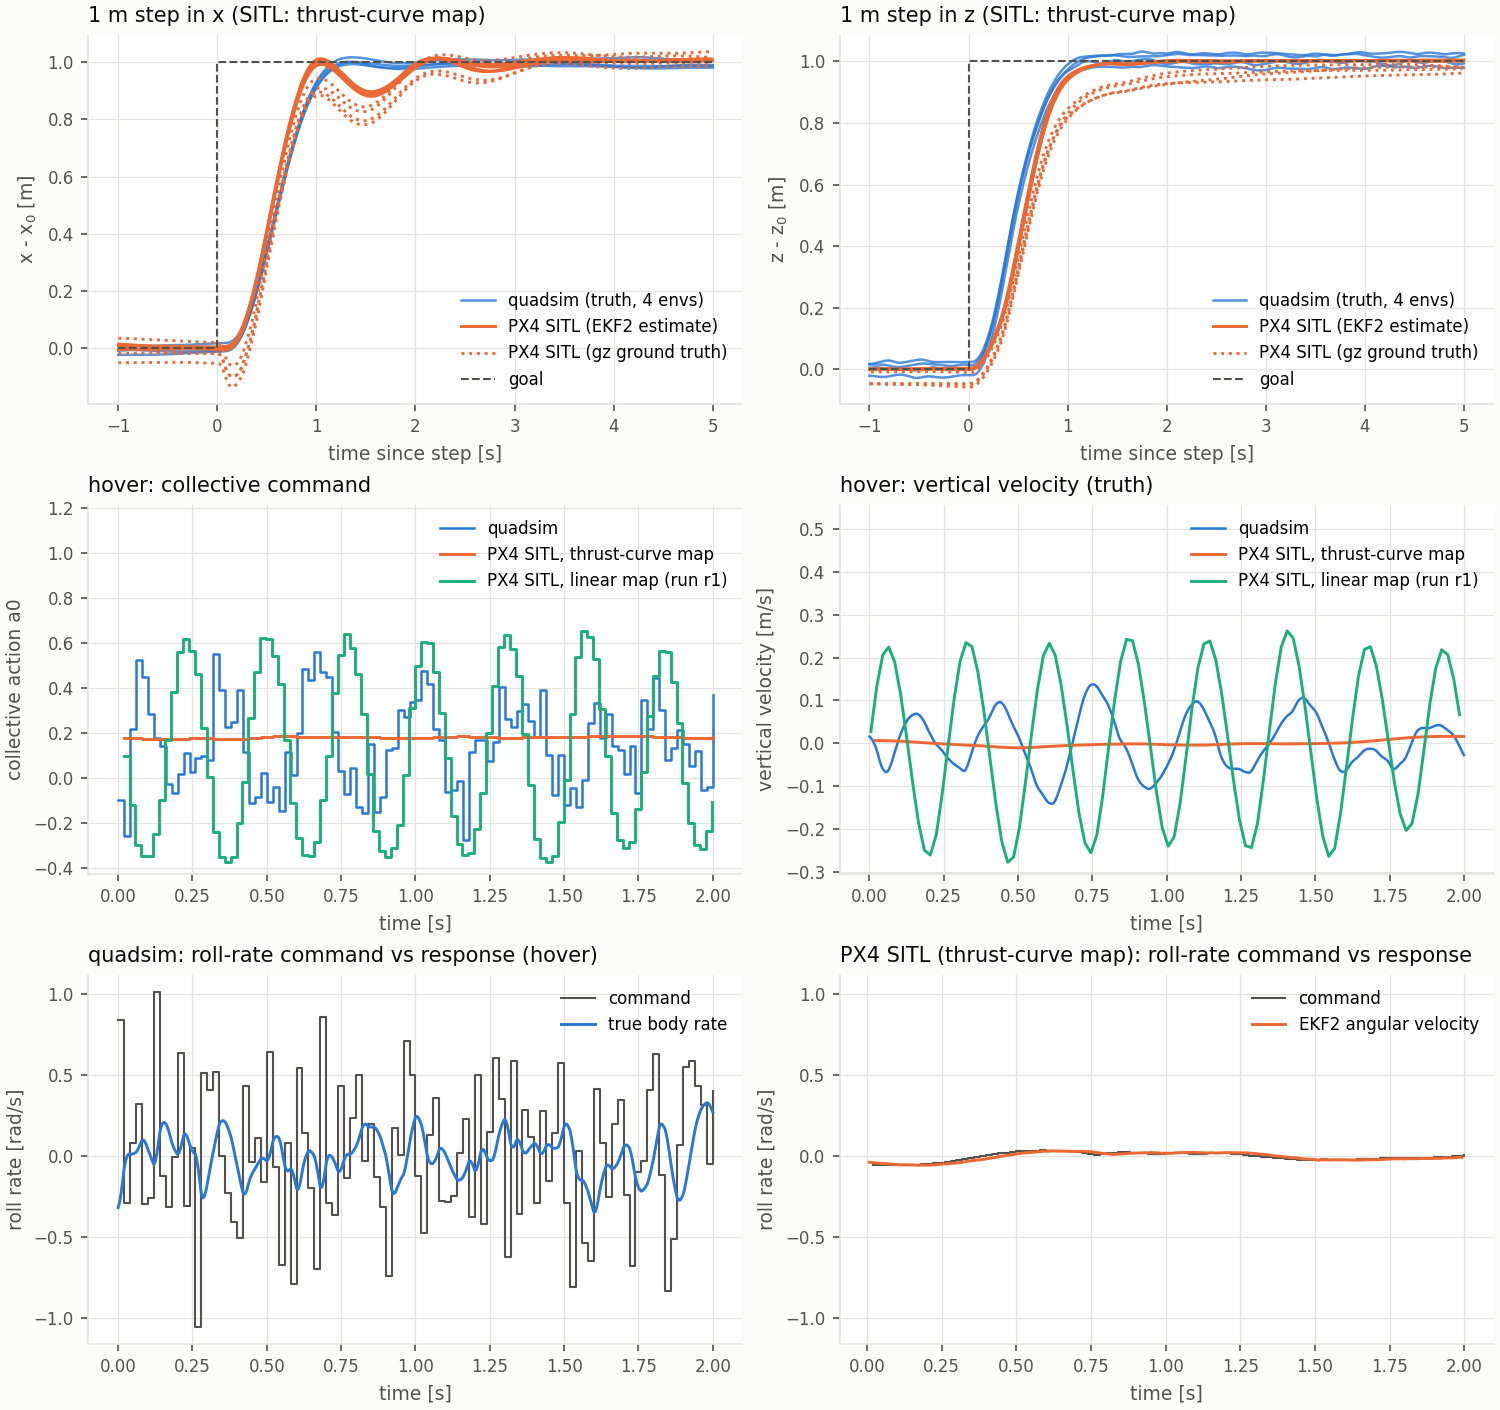
\includegraphics[width=\linewidth]{sitl_vs_quadsim.png}
\caption{Top: \SI{1}{m} steps (quadsim truth, SITL estimate and truth). Middle: hover collective command and vertical
velocity -- with the linear thrust map PX4 SITL shows a \SI{4}{Hz} heave limit cycle that the thrust-curve map removes.
Bottom: roll-rate command and response (quadsim commands chatter because of the white odometry noise).}
\label{fig:sitl-steps}
\end{figure}
Findings:
(i) \emph{Control performance transfers}: referenced to the estimate, SITL holds the pose to \SIrange{0.8}{1.0}{cm} RMS
(quadsim \SI{1.9}{cm}) and the $z$ step rises and settles as in quadsim; the smoother EKF2 estimate produces much quieter
commands than quadsim's white-noise odometry. (ii) The $x$ step settles slower in SITL (\SI{1.86}{s} vs \SI{1.07}{s}; the
position dips back to $\approx$\SI{0.9}{m}); the cause is not isolated (the pitch loop is not slower, see (iv)). (iii) \emph{Heave limit cycle}: with the
linear thrust map, 3 of 5 runs developed a persistent \SIrange{3.75}{4}{Hz} vertical oscillation (collective std 0.30--0.36,
vertical velocity 0.14--0.17\,m/s RMS) from the hand-over on; with the curve map 0 of 4 runs did. Quadsim shows the same
lightly damped mode as noise-driven heave; the 1.6$\times$ local thrust gain of the linear map turns it into a limit
cycle. (iv) \emph{Rate loop}: PX4's pitch response matches quadsim's delay (8--14 vs 13\,ms) with a smaller time constant
(38--44 vs 53\,ms); roll is slower (22--32\,ms) because the x500 airframe's allocation geometry
(\texttt{CA\_ROTOR*}=0.13/0.20--0.22\,m) differs from the gz rotor positions ($\pm$0.174\,m); setting the true geometry
reduced the roll delay by 4--12\,ms under matched conditions (2 runs). Fitted delays depend on the excitation by
$\pm$\SI{10}{ms} (closed-loop identification); with PX4's backward-differenced ground-truth rates all SITL delays appear
$\approx$\SI{10}{ms} longer. (v) PX4's hover-thrust estimate is 0.7295
(default \texttt{MPC\_THR\_HOVER} 0.60); without calibration ($s=1$, $-19\,\%$ thrust) the policy still flies but holds
\SI{1.3}{cm} low. (vi) Odometry is 5--16\,ms old at the policy step (median per run, max \SI{23}{ms}) -- at and above the
trained 0--10\,ms.

\subsection{Training distribution v1 and multi-seed comparison}\label{sec:v1}
The findings above define the v1 distribution (\cref{sec:dr}). Hover policies were trained with three seeds on v1 and
compared with three seeds of v0 (seed 42 plus two new seeds) in quadsim and in SITL (\cref{tab:hover-v1}).
\begin{table}[h]\centering\small
\resizebox{\linewidth}{!}{\begin{tabular}{lccc}\toprule
Metric & v0 (3 seeds) & v1 (3 seeds) & v2 (3 seeds)\\\midrule
quadsim, v0 distribution: success [\%] & 99.9 $\pm$ 0.0 & 99.7 $\pm$ 0.4 & 99.0 $\pm$ 0.6\\
quadsim, v0 distribution: final pos. error [cm] & 1.28 $\pm$ 0.07 & 1.83 $\pm$ 0.30 & 1.58 $\pm$ 0.12\\
quadsim, v1 distribution: success [\%] & 73.9 $\pm$ 2.0 & 74.4 $\pm$ 3.1 & 69.3 $\pm$ 5.7\\
quadsim, v1 distribution: final pos. error [cm] & 6.58 $\pm$ 0.12 & 6.77 $\pm$ 0.23 & 6.84 $\pm$ 0.14\\
quadsim, harsh OOD: success [\%] & 77.8 $\pm$ 1.2 & 66.0 $\pm$ 4.2 & 70.2 $\pm$ 2.0\\
quadsim, harsh OOD: crash [\%] & 3.7 $\pm$ 0.2 & 3.6 $\pm$ 0.4 & 3.4 $\pm$ 0.4\\
scenario $g=1.0$: hover RMS w.r.t. estimate [cm] & 1.87 $\pm$ 0.00 & 2.46 $\pm$ 0.32 & 1.95 $\pm$ 0.05\\
scenario $g=1.0$: collective std & 0.149 $\pm$ 0.016 & 0.211 $\pm$ 0.049 & 0.079 $\pm$ 0.003\\
scenario $g=1.6$: collective std & 0.209 $\pm$ 0.026 & 0.286 $\pm$ 0.079 & 0.112 $\pm$ 0.007\\
scenario $g=1.6$: vertical velocity RMS [cm/s] & 8.7 $\pm$ 1.0 & 9.0 $\pm$ 2.3 & 8.6 $\pm$ 0.8\\
SITL linear map: runs with limit cycle & 1 / 6 & 4 / 6 & 0 / 6\\
SITL curve map: runs with limit cycle & -- & 1 / 3 & 0 / 3\\
SITL linear map: collective std & 0.061 $\pm$ 0.080 & 0.310 $\pm$ 0.171 & 0.062 $\pm$ 0.016\\
SITL linear map: hover RMS w.r.t. estimate [cm] & 1.00 $\pm$ 0.10 & 2.17 $\pm$ 0.27 & 1.26 $\pm$ 0.23\\
SITL linear map: $x$ step settling [s] & 1.02 $\pm$ 0.02 & 1.05 $\pm$ 0.01 & 0.99 $\pm$ 0.05\\
SITL curve map: collective std & -- & 0.164 $\pm$ 0.142 & 0.031 $\pm$ 0.025\\
SITL curve map: hover RMS w.r.t. estimate [cm] & -- & 2.16 $\pm$ 0.74 & 1.29 $\pm$ 0.21\\
\bottomrule\end{tabular}
}
\caption{Hover policies trained on v0 vs v1, mean $\pm$ std over 3 seeds. Quadsim: 1000 episodes per seed and
condition; scenario: hover + steps with nominal dynamics and a thrust-map gain $g$ (1.6 = linear map on the gz x500).
SITL: limit-cycle runs = collective std $>0.1$ in hover. Source: \texttt{docs/results/hover\_v1.json}.}
\label{tab:hover-v1}
\end{table}
\TBD{v1 findings}

\subsection{Trajectory tracking and waypoints}
\Cref{tab:sitl-tasks} compares the tracking policy on a circle ($r=\SI{1}{m}$, \SI{0.2}{Hz}, \SI{1.26}{m/s}) and a figure-8
($r=\SI{1.5}{m}$, \SI{0.15}{Hz}) and the waypoint policy on a fixed 5-waypoint course, all with the thrust-curve map.
Referenced to the estimate, tracking in SITL equals quadsim (circle 2.2 vs \SI{2.5}{cm}, figure-8 3.4 vs \SI{3.0}{cm} RMSE);
the truth-referenced error is 3--4$\times$ larger because of EKF2's correlated error. The waypoint course was completed
in every SITL run (policy's own estimate-based switching) but took \SI{6.7}{s} instead of \SI{5.1}{s}; at up to
\SI{7}{m/s} EKF2's error reaches \SI{30}{cm}, so on truth some waypoints were passed just outside the \SI{0.3}{m} radius.
Removing quadsim's body drag did not change its time (\SI{5.13}{s}) and fixing the allocation geometry did not change
SITL's; PX4's saturation handling and slower inner loop are the remaining, not isolated, candidates.
\begin{table}[h]\centering\small
\begin{tabular}{llcc}\toprule
Task & Metric & quadsim & PX4 SITL\\\midrule
Tracking, circle (r 1 m, 0.2 Hz) & RMSE truth [cm] & 1.8 $\pm$ 0.4 & 6.3 $\pm$ 0.7\\
 & RMSE w.r.t. estimate [cm] & 2.5 $\pm$ 0.1 & 2.2 $\pm$ 0.2\\
Tracking, figure-8 (r 1.5 m, 0.15 Hz) & RMSE truth [cm] & 2.7 $\pm$ 0.2 & 9.2 $\pm$ 0.4\\
 & RMSE w.r.t. estimate [cm] & 3.0 $\pm$ 0.1 & 3.4 $\pm$ 0.4\\
Waypoints (5) & course completed & 1.00 & 1.00\\
 & time to finish [s] & 5.13 $\pm$ 0.02 & 6.74 $\pm$ 0.27\\
 & estimate error during course, RMS [cm] & -- & 15.2 $\pm$ 0.7\\
\bottomrule\end{tabular}

\caption{Tracking and waypoint policies (v0), quadsim (32 envs) vs PX4 SITL (2 runs each); RMSE after the first
\SI{2}{s}. Source: \texttt{docs/results/sitl\_tasks.json}.}
\label{tab:sitl-tasks}
\end{table}

\subsection{Obstacle navigation through the velocity interface}
The range-ring navigation policy commands velocities, which PX4's position controller tracks. Obstacles are virtual in
SITL: a 2-D LiDAR node ray-casts the training ring against the cylinders of a layout from the ground-truth pose (identical
to the training caster, unit-tested), and collisions are evaluated from the ground truth with the training criterion. Six
layouts drawn from the full-density training distribution were flown once in SITL and by 32 quadsim environments each
(\cref{tab:sitl-nav}). With PX4's default velocity controller only 2 of 6 SITL flights reached the goal, against 87\,\%
quadsim success on the same layouts. Identifying both velocity loops from the flight data explains the gap: PX4's
lateral velocity response has $L=\SI{0.22}{s}$, $\tau=\SI{0.44}{s}$ (VAF 0.85) against $L=\SI{0.14}{s}$, $\tau=\SI{0.22}{s}$
for quadsim's simulated cascade -- PX4's default horizontal velocity gain (\texttt{MPC\_XY\_VEL\_P\_ACC}=1.8) is lower than the
simulated one (3.0), so avoidance manoeuvres arrive late. Configuring PX4's velocity controller like the training cascade
(\texttt{MPC\_XY\_VEL\_P\_ACC}=3.0, D=0, \texttt{MPC\_Z\_VEL\_I\_ACC}=1.0, tilt limit 0.6\,rad) reduced the lateral time constant
to \SI{0.25}{s} (quadsim \SI{0.22}{s}) and doubled the SITL success to 4 of 6 layouts; the remaining failures are layout~1
(hard in quadsim as well, 38\,\% success) and layout~4. The residual lateral delay ($\approx$\SI{0.21}{s} vs \SI{0.14}{s})
comes from PX4's attitude and rate chain and is not represented in training. With one SITL flight per layout these rates
are indicative only; the lesson for deployment is that velocity-interface policies must be trained with the target
autopilot's velocity-loop dynamics (identified, or randomized over a range that contains them).
\begin{table}[h]\centering\small
\resizebox{\linewidth}{!}{\begin{tabular}{ccccc}\toprule
Layout & obstacles & quadsim success / collision [\%] & PX4 default velocity loop & PX4 velocity loop matched to quadsim\\\midrule
0 & 7 & 100 / 0 & goal & goal\\
1 & 15 & 38 / 62 & collision & collision\\
2 & 13 & 97 / 3 & goal & goal\\
3 & 15 & 97 / 3 & collision & goal\\
4 & 11 & 91 / 6 & collision & collision\\
5 & 15 & 100 / 0 & collision & goal\\
\bottomrule\end{tabular}
}
\caption{Navigation layouts: quadsim success / collision rate (32 envs per layout) and the outcome of the PX4 SITL flight
with PX4's default and with a quadsim-matched velocity controller. Source: \texttt{docs/results/sitl\_tasks.json}.}
\label{tab:sitl-nav}
\end{table}

\subsection{Summary of the cross-check}
\begin{itemize}
\item All CTBR policies (hover, tracking, waypoints) fly PX4 SITL as offboard controllers; at the level the policy
controls (estimate-referenced) their performance matches quadsim; the bridge's safety gating is verified.
\item Sim-to-sim gaps were found and quantified, each with an identified cause: EKF2's correlated error (training model too
white), GNSS delay mis-configuration in SITL, the thrust-map nonlinearity (heave limit cycle; fixed by the curve map),
PX4's roll/pitch-asymmetric rate loop (allocation geometry), up to \SI{20}{ms} observation age, and -- the
largest -- PX4's slower velocity loop for the velocity-interface navigation policy.
\item Not done: hardware flights, depth/RGB policies in SITL (needs a rendered camera in gz), retraining the
navigation policy with a randomized velocity loop.
\end{itemize}
